\section{Equivalent problems}
Many algorithms do not solve the originally stated minimum cost flow problem, but rather similar problems that are equivalent to the original. 
% In this section, we present some variants of the problem and show that they are equivalent to the original.

\subsection{Minimum cost circulation with lower bounds}
Let us introduce a minimum cost circulation. Some of the algorithms in the paper are tailored to exactly this kind of problem.
We introduce a definition with flow lower bounds on the arcs. Let $G=(V,E)$ be a directed network with costs $c_{ij}$, capacities $u_{ij}$ and lower-bounds $l_{ij}$ for each arc $(i,j) \in E$.

\begin{defn}[Circulation with lower bounds \cite{williamson2019}]
    A \textbf{circulation with lower bounds} $x: E \rightarrow \mathbb{R}^{\geq 0}$ is an assignment of nonnegative reals to the arcs such that the following two properties are obeyed:
    \begin{itemize}
        \item for all edges $(i,j) \in E$, \[
        l_{ij}\leq x_{ij} \leq u_{ij},
        \]
        \item for all $i\in V$, the total flow entering $i$ is equal to the flow leaving i; that is, \[
        \sum_{k\colon (k,i)\in E}x_{ki} =  \sum_{k\colon (i,k)\in E}x_{ik}\text{.}
        \]
    \end{itemize}
    The cost of the circulation is $c(x) = \sum_{(i,j)\in E} c_{ij}x_{ij}$.
\end{defn}
\begin{defn}[Minimum cost circulation with lower bounds \cite{williamson2019}]
    The \textbf{minimum cost circulation problem with lower bounds}  can be stated as follows: \[\text{minimize}\ c(x) = \sum_{(i,j)\in E} c_{ij}x_{ij}\]
    among all circulations with lower bounds.
\end{defn}

\begin{theorem}
    The minimum cost flow problem and the minimum cost circulation problem are equivalent.
\end{theorem}

\begin{proof}[Proof (see {\cite[p.~111]{williamson2019}})]
    $(\Rightarrow)$ Given an instance of the minimum cost flow, we convert it to an instance of the minimum cost circulation problem. Add node $s$ to the graph. For any $i \in V$ such that $b(i) > 0$, we create an arc $(s,i)$ with $c_{si} = 0$ and $l_{si} = u_{si} = b(i)$. For any supply node $j\in V$ (with $b(i)< 0$), we create an arc $(j,s)$, with $l_{js} = u_{js} = -b(j)$ and cost $c_{js} = 0$. It is easy to see that the optimal costs are the same. The reduction is presented in \Cref{fig:mcf_to_mcc}. 

    $(\Leftarrow)$ If we want to create a minimum cost flow instance from a circulation, we need to remove the lower-bounds of the flow from the arcs. To do this, we implicitly assume that the arc $(i,j)$ already contains $l_{ij}$ units of flow. Therefore, the imbalance $b(i)$ decreases by $l_{ij}$, and $b(j)$ increases by $l_{ij}$.
    In other words, we perform the following operations.  Let $x_{ij}' = x_{ij} - l_{ij}$, and $u_{ij}' = u_{ij} - l_{ij}$. Then, set $b(i) = \sum_{k\colon (k,i)\in E} l_{ki} - \sum_{k\colon (i,k) \in  E} l_{ik}$. Given a feasible circulation $x$ in the original problem, we get a feasible flow $x'$ for a minimum cost flow problem with the same costs, capacity $u'$ and imbalance $b$. It is easy to see that the operations preserve optimality.

\end{proof}

\begin{figure}[H]
    \centering
    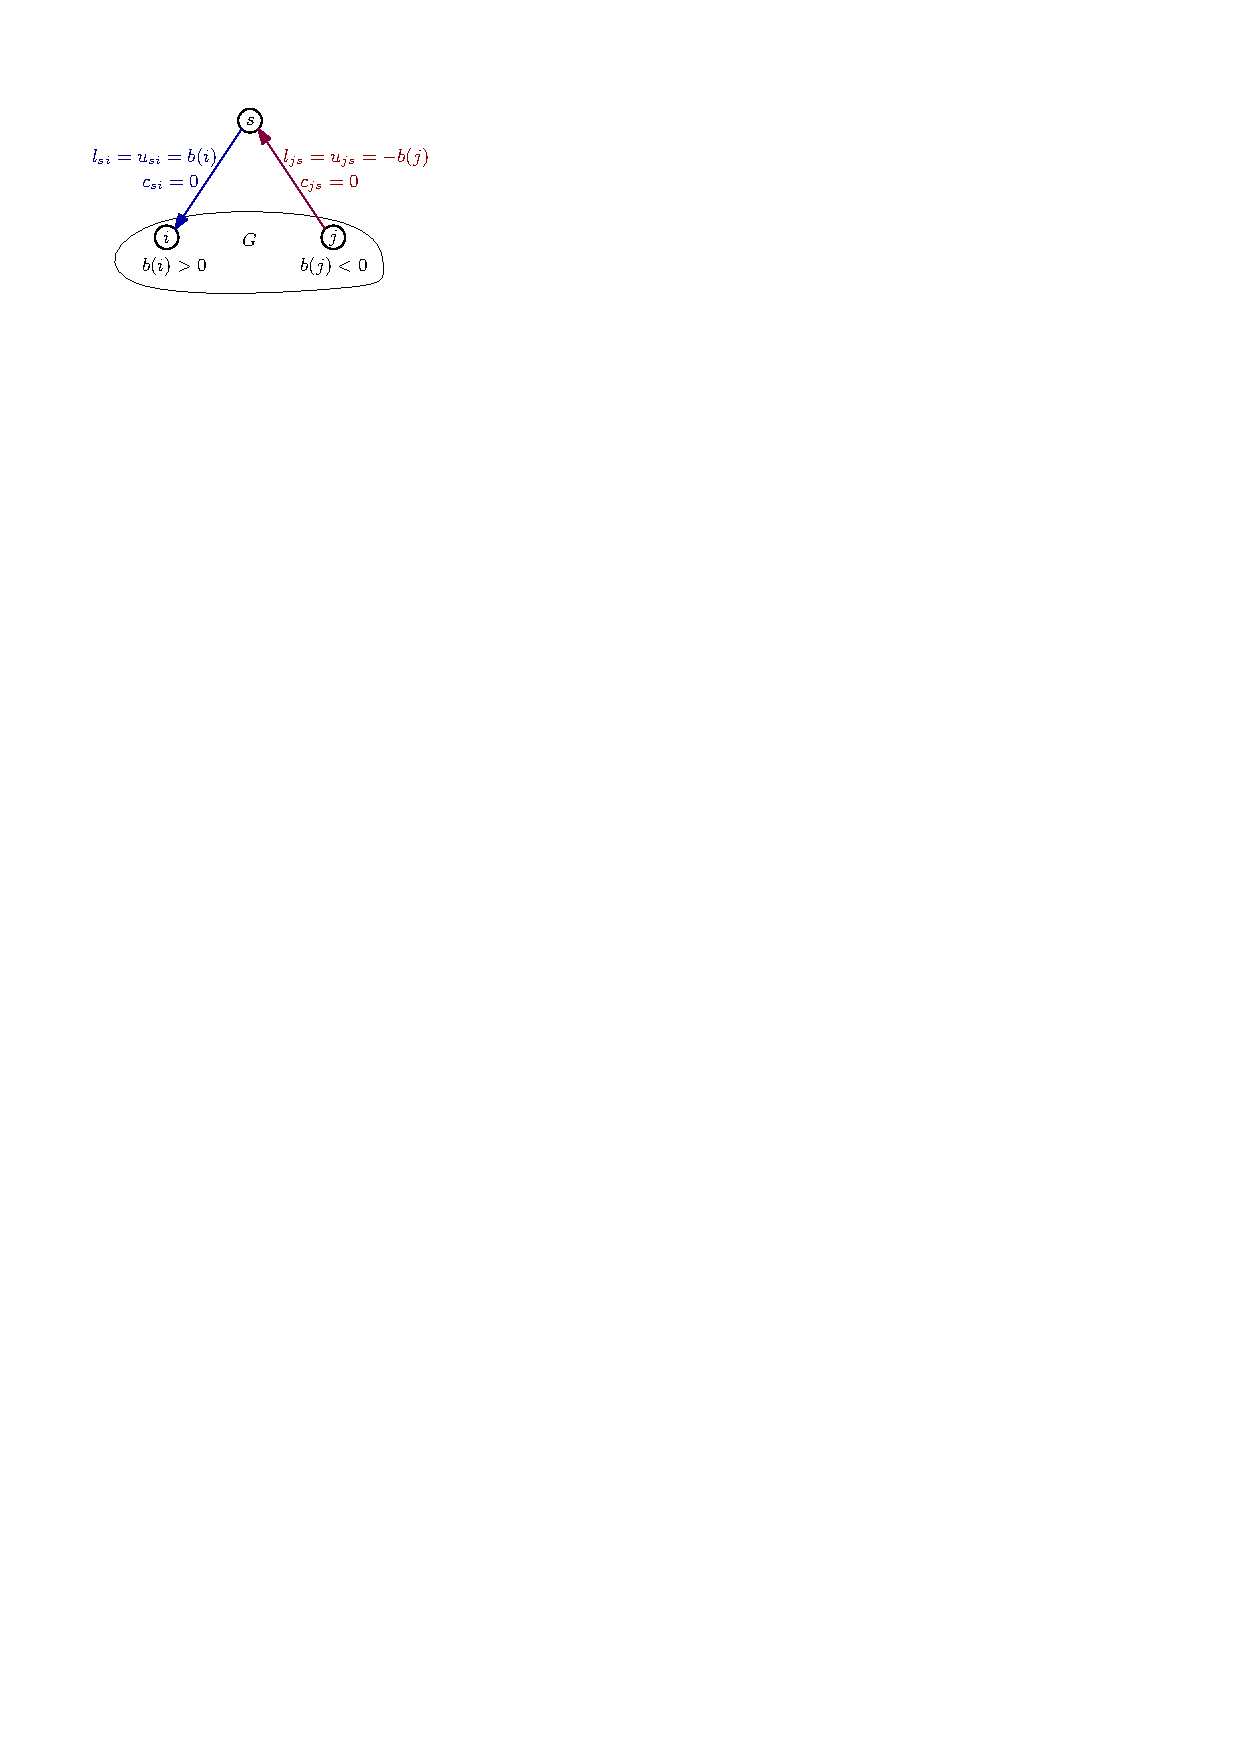
\includegraphics[width=0.5\linewidth]{chapters/introduction/img/mcc.pdf}
    \caption{Reduction from minimum cost flow to minimum cost circulation problem.}
    \label{fig:mcf_to_mcc}
\end{figure}

\subsection{Minimum cost circulation without lower bounds}\label{sec:mcc_nolower}
Then we redefine the problem to remove lower bounds from the definition. It is more convenient to work with capacities only, and many algorithm descriptions for the minimum cost circulation problem uses this definition for simplicity. 

\begin{defn}[Circulation \cite{williamson2019}]
A \textbf{circulation} $x: E \to \mathbb{R}$ is an assignment of reals to the arcs such that the following three properties are obeyed:
    \begin{itemize}
        \item for all arcs $(i,j)\in E$, \[x_{ij} \leq u_{ij},\]
        \item for all $i\in V$, the total flow leaving $i$ is zero; that is, \[
        \sum_{k\colon(i,k) \in E} x_{ik} =0,
        \]
        \item for all $(i,j) \in E$ \[
        x_{ij} = -x_{ji}.
        \]
    \end{itemize}
\end{defn}

\begin{defn}[Minimum cost circulation \cite{williamson2019}]
    The \textbf{minimum cost circulation} can be stated as follows:
    \[
    \text{minimize }c(x) = \frac{1}{2}\sum_{(i,j)\in E} c_{ij}x_{ij} 
    \]
    among all circulations.
\end{defn}

Notice that the flow in the arc is taken twice ($x_{ij}$ and $x_{ji}$), this is why we divide the cost in half .

We perform the reduction as follows. Let $G = (V, E)$ be the original network with lower-bounded arcs. We create a new network $G' = (V, E')$ that has no lower bounds, using only upper bounds $u_{ij}'$ for each arc $(i,j) \in E'$. 

For every original arc $(i, j) \in E$, we set the upper bound to $u_{ij}' = u_{ij}$. We then add a backward arc $(j, i)$ with an upper bound of $u_{ji}' = -l_{ij}$. 

By definition, flow is skew-symmetric, meaning $x_{ij}' = -x_{ji}'$. Because of this, if the backward flow is within its upper bound ($x_{ji}' \leq u_{ji}'$), we have $-x_{ij}' \leq -l_{ij}$. Multiplying both sides by $-1$ gives $x_{ij}' \geq l_{ij}$, which shows that the original lower bound requirement is met.

We have the similar optimality conditions for the minimum cost circulation as for minimum cost flow problem described in \Cref{sec:optimality_conditions_flow}.
\begin{theorem}[Theorem 5.3 in \cite{williamson2019}]
    Let $G(x)$ be a residual network for a graph $G$ a circulation $x$. 
    The following statements are equivalent for $x$:
    \begin{enumerate}
        \item $x$ is a minimum-cost circulation,
        \item there is no negative-cost cycle in $G(x)$,
        \item there are potentials $\pi$ such that $c_{ij}^\pi \geq 0$ for all arcs $(i,j)$ in $G(x)$.
    \end{enumerate}
\end{theorem}

\subsection{Uncapacitated minimum cost flow}
\label{sec:uncapacitated}
Since the arc capacities impose certain restrictions, there are algorithms designed to solve a simpler version of the minimum cost flow problem, with no capacities associated with the arcs. In this subsection, we present a well-known reduction from the capacitated minimum cost flow problem to the uncapacitated one.

Suppose that we have a capacitated network $G=(V,E)$. Let $G'=(V', E')$ be the new network with supply/demand $b'$, arc costs $c'$ and no capacities. We perform the following reduction. Let $(i,j) \in E$ be an arc with capacity $u_{ij}$ and cost $c_{ij}$. We introduce an additional node $k$ and replace arc $(i,j)$ with two arcs $(i,k)$ and $(j,k)$ as it is shown in \Cref{fig:uncapacitated}. 

\begin{figure}[H]
    \centering
    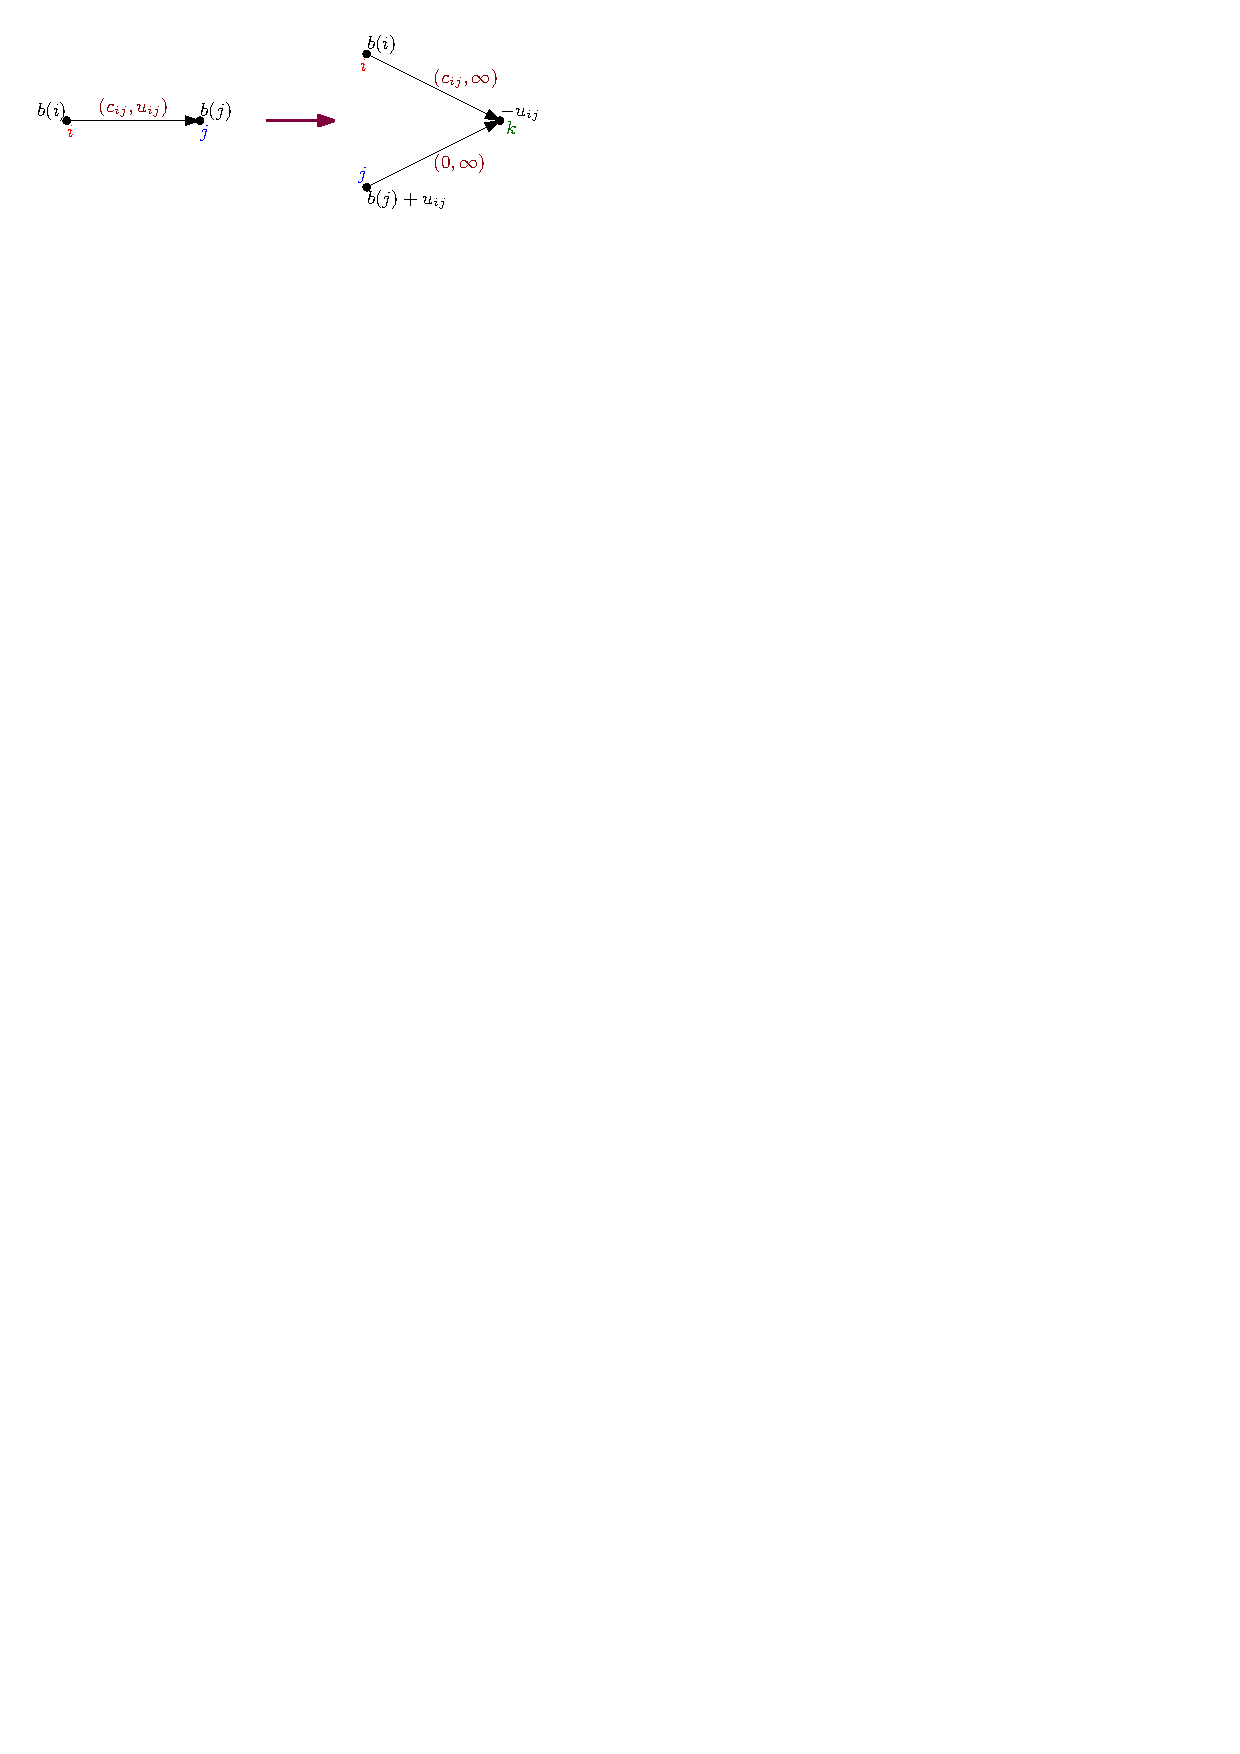
\includegraphics[width=0.8\linewidth]{chapters/introduction/img/uncapacitated.pdf}
    \caption{Reduction from capacitated to uncapacitated network.}
    \label{fig:uncapacitated}
\end{figure}

Now we provide some justification of the reduction. Suppose that the flow $x_{ij}$ on arc $(i,j)\in E$ is some arbitrary number $0 \leq a \leq u_{ij}$, and that $e(i) = b(i)-a$, $e(j) = b(j)+a$. Let $e'\colon V' \to \mathbb{R}$ denote an excess for uncapacitated network $G'$. We show that the excesses in the uncapacitated network match the original. 

Initially we let $e'(i) \coloneq b(i)$ and $e'(j) \coloneq b(j)$. To get the same cost, we need to push $a$ units of flow through the edge $(i,k) \in E'$. Now we have $e'(i)=b(i) -a$ and $e'(k) = -u_{ij} + a$. To enforce feasibility, the only option is to send $u_{ij} - a$ units of flow through the arc $(j,k)\in E'$. Therefore, we have equity $e(j) = b(j) + u_{ij} - (u_{ij} - a) = b(j) + a$ as in the capacitated case.